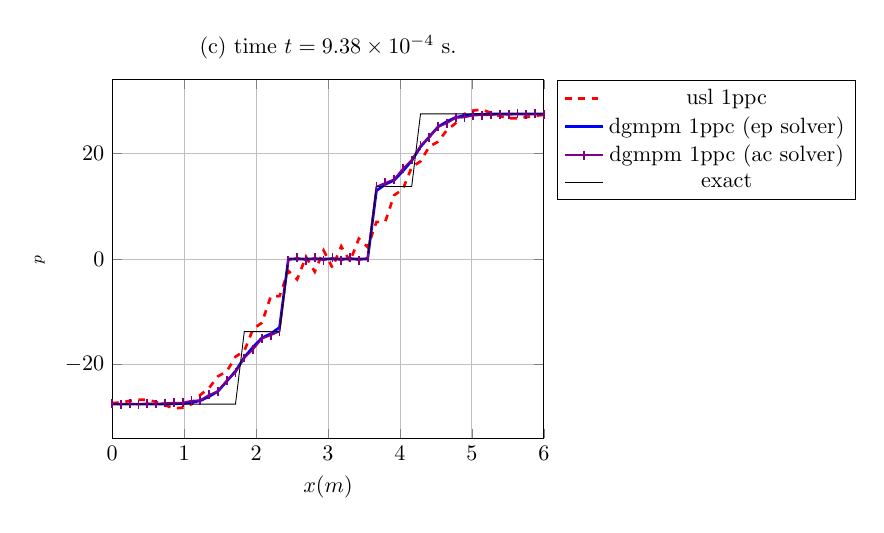
\begin{tikzpicture}[scale=0.8]
\begin{axis}[xlabel=$x (m)$,ylabel=$\eps^p$,ymajorgrids=true,xmajorgrids=true,legend pos=outer north east,title={(c) time $t = 9.38\times 10^{-4} $ s.},xmin=0.,xmax=6.]
\addplot[Red,very thick,mark=none,dashed] coordinates {(0.0,-27.331872449853556) (0.12244897959183673,-27.174400085417467) (0.24489795918367346,-26.904779830121768) (0.36734693877551017,-26.69301343005911) (0.4897959183673469,-26.683543140751915) (0.6122448979591837,-27.106963962300345) (0.7346938775510203,-27.704030887608354) (0.8571428571428571,-28.33906014232905) (0.9795918367346939,-28.167172814076366) (1.1020408163265305,-27.53334986092529) (1.2244897959183674,-25.775044707062726) (1.346938775510204,-24.466615882102165) (1.4693877551020407,-22.247186500301964) (1.5918367346938775,-21.33079179039491) (1.7142857142857142,-18.523714044368063) (1.836734693877551,-17.44233776410034) (1.9591836734693877,-13.237799741628182) (2.0816326530612246,-12.0894356407598) (2.204081632653061,-7.096371776087362) (2.326530612244898,-7.032925295785245) (2.4489795918367347,-2.2620897664972315) (2.571428571428571,-3.858668388515009) (2.693877551020408,0.4300541105363164) (2.816326530612245,-2.410115988529146) (2.9387755102040813,1.6326922086221445) (3.061224489795918,-1.6326922086221325) (3.183673469387755,2.410115988529122) (3.306122448979592,-0.43005411053631265) (3.4285714285714284,3.858668388514974) (3.5510204081632653,2.2620897664972395) (3.673469387755102,7.032925295785231) (3.7959183673469385,7.096371776087392) (3.9183673469387754,12.089435640759786) (4.040816326530612,13.237799741628214) (4.163265306122449,17.442337764100337) (4.285714285714286,18.523714044368088) (4.408163265306122,21.330791790394894) (4.530612244897959,22.247186500301982) (4.653061224489796,24.466615882102147) (4.775510204081632,25.775044707062744) (4.8979591836734695,27.53334986092529) (5.020408163265306,28.167172814076363) (5.142857142857142,28.33906014232903) (5.26530612244898,27.70403088760834) (5.387755102040816,27.106963962300348) (5.5102040816326525,26.683543140751933) (5.63265306122449,26.693013430059132) (5.755102040816326,26.904779830121797) (5.877551020408163,27.17440008541749) (6.0,27.331872449853574) };
\addplot[Blue,very thick,mark=none,solid] coordinates {(0.0,-27.517363397075158) (0.12244897959183673,-27.51732379155038) (0.24489795918367346,-27.517228936294842) (0.36734693877551017,-27.516689788484122) (0.4897959183673469,-27.51556852970287) (0.6122448979591837,-27.51025382248486) (0.7346938775510203,-27.500198710367762) (0.8571428571428571,-27.46081288016468) (0.9795918367346939,-27.394149463815687) (1.1020408163265305,-27.182111927326964) (1.2244897959183674,-26.86831399158136) (1.346938775510204,-26.07814929006618) (1.4693877551020407,-25.08839352872312) (1.5918367346938775,-23.189519000405884) (1.7142857142857142,-21.27348955232935) (1.836734693877551,-18.64183859399968) (1.9591836734693877,-16.67485639518814) (2.0816326530612246,-14.95207519835609) (2.204081632653061,-14.149762008703409) (2.326530612244898,-12.971197310204563) (2.4489795918367347,3.556080111931078e-14) (2.571428571428571,1.8614128550443383e-14) (2.693877551020408,1.1448988934369504e-14) (2.816326530612245,3.15403661725491e-14) (2.9387755102040813,2.1706952110207872e-14) (3.061224489795918,1.837643246978256e-14) (3.183673469387755,7.175699018437745e-15) (3.306122448979592,1.6868189305533344e-14) (3.4285714285714284,1.74998305367758e-14) (3.5510204081632653,1.3502410778036318e-14) (3.673469387755102,12.971197310204614) (3.7959183673469385,14.149762008703469) (3.9183673469387754,14.952075198356113) (4.040816326530612,16.67485639518816) (4.163265306122449,18.641838593999687) (4.285714285714286,21.273489552329384) (4.408163265306122,23.189519000405888) (4.530612244897959,25.088393528723138) (4.653061224489796,26.07814929006618) (4.775510204081632,26.868313991581342) (4.8979591836734695,27.182111927326957) (5.020408163265306,27.3941494638157) (5.142857142857142,27.46081288016466) (5.26530612244898,27.500198710367762) (5.387755102040816,27.51025382248485) (5.5102040816326525,27.515568529702865) (5.63265306122449,27.51668978848415) (5.755102040816326,27.517228936294806) (5.877551020408163,27.517323791550382) (6.0,27.517363397075165) };
\addplot[Purple,thick,mark=|,solid] coordinates {(0.0,-27.455491898583844) (0.12244897959183673,-27.52990791746212) (0.24489795918367346,-27.39669410111553) (0.36734693877551017,-27.56069772218648) (0.4897959183673469,-27.354208534961813) (0.6122448979591837,-27.484169218141297) (0.7346938775510203,-27.30529154707286) (0.8571428571428571,-27.260887430891447) (0.9795918367346939,-27.234362200737557) (1.1020408163265305,-26.87048565463221) (1.2244897959183674,-26.76603983934888) (1.346938775510204,-25.75807449243556) (1.4693877551020407,-25.06955937174821) (1.5918367346938775,-23.02673771458467) (1.7142857142857142,-21.509235536573875) (1.836734693877551,-18.773874989550777) (1.9591836734693877,-17.141311478227397) (2.0816326530612246,-15.098912535609557) (2.204081632653061,-14.451161421148855) (2.326530612244898,-13.715612700621918) (2.4489795918367347,-0.23693029878140853) (2.571428571428571,0.24220658661539068) (2.693877551020408,-0.22882318056987147) (2.816326530612245,0.2316928153217551) (2.9387755102040813,-0.22713962166300733) (3.061224489795918,0.22713962166305024) (3.183673469387755,-0.2316928153217785) (3.306122448979592,0.22882318056992768) (3.4285714285714284,-0.24220658661539307) (3.5510204081632653,0.23693029878141705) (3.673469387755102,13.71561270062201) (3.7959183673469385,14.451161421148875) (3.9183673469387754,15.098912535609603) (4.040816326530612,17.141311478227408) (4.163265306122449,18.77387498955077) (4.285714285714286,21.509235536573904) (4.408163265306122,23.026737714584694) (4.530612244897959,25.06955937174818) (4.653061224489796,25.758074492435522) (4.775510204081632,26.766039839348913) (4.8979591836734695,26.870485654632194) (5.020408163265306,27.23436220073757) (5.142857142857142,27.260887430891422) (5.26530612244898,27.305291547072898) (5.387755102040816,27.484169218141297) (5.5102040816326525,27.354208534961796) (5.63265306122449,27.560697722186475) (5.755102040816326,27.39669410111557) (5.877551020408163,27.529907917462097) (6.0,27.455491898583855) };
\addplot[black,thin,mark=none,solid] coordinates {(0.0,-27.517375820951077) (0.12244897959183673,-27.517375820951077) (0.24489795918367346,-27.517375820951077) (0.36734693877551017,-27.517375820951077) (0.4897959183673469,-27.517375820951077) (0.6122448979591837,-27.517375820951077) (0.7346938775510203,-27.517375820951077) (0.8571428571428571,-27.517375820951077) (0.9795918367346939,-27.517375820951077) (1.1020408163265305,-27.517375820951077) (1.2244897959183674,-27.517375820951077) (1.346938775510204,-27.517375820951077) (1.4693877551020407,-27.517375820951077) (1.5918367346938775,-27.517375820951077) (1.7142857142857142,-27.517375820951077) (1.836734693877551,-13.758687910475539) (1.9591836734693877,-13.758687910475539) (2.0816326530612246,-13.758687910475539) (2.204081632653061,-13.758687910475539) (2.326530612244898,-13.758687910475539) (2.4489795918367347,-0.0) (2.571428571428571,-0.0) (2.693877551020408,-0.0) (2.816326530612245,-0.0) (2.9387755102040813,-0.0) (3.061224489795918,-0.0) (3.183673469387755,-0.0) (3.306122448979592,-0.0) (3.4285714285714284,-0.0) (3.5510204081632653,-0.0) (3.673469387755102,13.758687910475539) (3.7959183673469385,13.758687910475539) (3.9183673469387754,13.758687910475539) (4.040816326530612,13.758687910475539) (4.163265306122449,13.758687910475539) (4.285714285714286,27.517375820951077) (4.408163265306122,27.517375820951077) (4.530612244897959,27.517375820951077) (4.653061224489796,27.517375820951077) (4.775510204081632,27.517375820951077) (4.8979591836734695,27.517375820951077) (5.020408163265306,27.517375820951077) (5.142857142857142,27.517375820951077) (5.26530612244898,27.517375820951077) (5.387755102040816,27.517375820951077) (5.5102040816326525,27.517375820951077) (5.63265306122449,27.517375820951077) (5.755102040816326,27.517375820951077) (5.877551020408163,27.517375820951077) (6.0,27.517375820951077) };
\legend{usl 1ppc,dgmpm 1ppc (ep solver),dgmpm 1ppc (ac solver),exact}
\end{axis}
\end{tikzpicture}
%%% Local Variables:
%%% mode: latex
%%% TeX-master: "../../mainManuscript"
%%% End:
